\documentclass[a4paper, 12pt, twoside]{article}
\usepackage{estilo}
\EnableReviewColors % Comente esta linha para remover as cores

\title{Título do resumo}

\author{%
  \reviewcolor{red}{Preencher nomes e emails apenas após aprovação}\\
  Nome autor principal\authorinfo{autor-principal@email.com} \\
  Nome coautor, um por linha, orientador por último\authorinfo{coautor1@email.com}
}
\date{}

\begin{document}
\maketitle

\reviewcolor{orange}{
\noindent \textbf{Esse preâmbulo colorido} não faz parte dos elementos textuais. Ele está aqui apenas para informar a natureza do resumo expandido e informações importantes. Deve ser removido antes da submissão. A formatação é aplicada automaticamente pelo \LaTeX. Não altere manualmente a formatação do texto, dos títulos, das margens, das citações, das tabelas ou das figuras.
}

\reviewcolor{red}{
\noindent \textbf{Leia todo o modelo antes de escrever:} ele foi elaborado como um guia de formatação e também de escrita científica. Cada seção indica qual conteúdo deve ser inserido e apresenta erros comuns de escrita.
}

\reviewcolor{purple}{
\noindent \textbf{O resumo expandido} deve ser utilizado \textbf{exclusivamente} para trabalhos que possuam características de um trabalho científico. O trabalho deve apresentar, de forma estruturada e articulada, um problema ou questão investigativa, objetivos, procedimentos metodológicos, resultados e conclusões. O texto \textbf{deve possuir de 3 a 5 páginas}. Não respeitar os limites pode implicar em \textbf{reprovação}.
}

\reviewcolor{brown}{
\noindent \textbf{Ferramentas de IA} generativa podem ser utilizadas como apoio à organização de ideias, revisão, tradução e aprimoramento da redação. Os autores permanecem responsáveis pelo conteúdo e devem verificar as informações, dados, referências e afirmações produzidas ou sugeridas por essas ferramentas.
}

\reviewcolor{orange}{
\noindent \textbf{Relatos de experiência} que consistam exclusivamente na descrição de atividades realizadas, sem investigação ou análise sistemática, devem ser submetidos como resumo simples, na trilha correspondente.
}

%%%%%%%%%%%%%%%%%%%%% RESUMO E ABSTRACT %%%%%%%%%%%%%%%%%%%%%%%%%%%%%%

\qabstract{Resumo}{Palavras-chave}{ODS}{% Mantenha esse % colado no {
O resumo é a apresentação concisa dos pontos relevantes de um documento. Deve ressaltar o objetivo, o método, os resultados e as conclusões do documento. É uma sequência de frases concisas, afirmativas e não de enumeração de tópicos. Não deve ter indentação ou parágrafos. Deve apresentar o tema principal do documento e, quando pertinente, informar a categoria do
tratamento, como pesquisa, estudo de caso ou outra modalidade de investigação. O verbo deve estar na voz ativa e na terceira pessoa do singular. A extensão
do resumo deve ser de 100 a 250 palavras.
}{ % Palavras-chave
Informe de três a cinco palavras-chave ou expressões curtas diretamente relacionadas ao conteúdo do trabalho. Inicie cada palavra-chave com letra minúscula, exceto substantivos próprios e nomes científicos, e separe-as por \textbf{ponto e vírgula}.
}{ % Objetivos ODS
Informe apenas um Objetivo de Desenvolvimento Sustentável (ODS), utilizando a nomenclatura oficial em letra minúscula. Consulte \url{https://brasil.un.org/pt-br/sdgs}
}

\qabstract{Abstract}{Keywords}{SDG}{% Mantenha esse % colado no {
O abstract é a versão integral do resumo traduzido para inglês. Também as palavras-chave e o ODS devem ser traduzidos adequadamente.
}{ % Keywords
palavra-chave 1. palavra-chave 2. palavra-chave 3. palavra-chave opcional.
}{ % Objetivos ODS em inglês
Escolher um dos tópicos em \url{https://sdgs.un.org/goals}
}

%%%%%%%%%%%%%%%%%%%%%%%%%%%%%% SEÇÕES %%%%%%%%%%%%%%%%%%%%%%%%%%%%%

\section{Introdução}

Parte inicial do resumo, deve delimitar o tema e apresentar o problema, a
justificativa e os objetivos da pesquisa. Deve situar o leitor no contexto do
trabalho, indicando, quando pertinente, a lacuna ou questão que motiva a
investigação e as questões de pesquisa ou hipóteses adotadas. Deve apresentar
brevemente a abordagem metodológica, sem substituir sua descrição detalhada
na seção de metodologia. Os elementos apresentados devem estar articulados
entre si e com as demais partes do trabalho. A fundamentação teórica necessária para contextualizar e sustentar o problema deve ser apresentada na seção correspondente, com as devidas citações. Evite antecipar resultados ou conclusões.

Esse parágrafo é um exemplo de como inserir um citação curta: \enquote{Esse é um texto de citação curta inserido diretamente no fluxo de leitura.} Esse é um exemplo de inserção de referência bibliográfica \cite{bittar2001linguagem}.

\begin{quote}
Esse é um exemplo de citação longa: a citação direta com mais de três linhas deve ser destacada com recuo de 4 cm da margem esquerda, em letra menor do que a utilizada no texto (tamanho 10), sem as aspas e com espaçamento simples entrelinhas. A citação deverá ser separada do texto que a precede [...] \cite{ufc2017guia}.
\end{quote}

\section{Desenvolvimento}

Parte que contém a exposição ordenada e pormenorizada do assunto tratado.
Deve ser dividido em subseções. A subseção de Fundamentação teórica pode ser omitida quando não for necessária, porém Metodologia e Resultados e Discussão são essenciais do trabalho científico. Outra subseções podem ser criadas caso julgar adequado. Esse é um exemplo de como citar uma bibliografia, conforme a NBR 6024 (ABNT, 2012) \cite{Mauricio}.

\subsection{Fundamentação Teórica}

Apresente os conceitos, teorias e trabalhos anteriores necessários para
contextualizar e fundamentar a investigação. Priorize referências diretamente
relacionadas ao problema e aos objetivos do trabalho. A fundamentação deve
sustentar a análise realizada, evitando a apresentação de informações que não
contribuam para a compreensão ou discussão dos resultados.

A Figura \ref{fig:algo} é apenas um exemplo de como inserir e citar uma figura.

\begin{figure}[!ht]
\caption{Título da Imagem}
\label{fig:algo}
\centering % para centralizarmos a figura
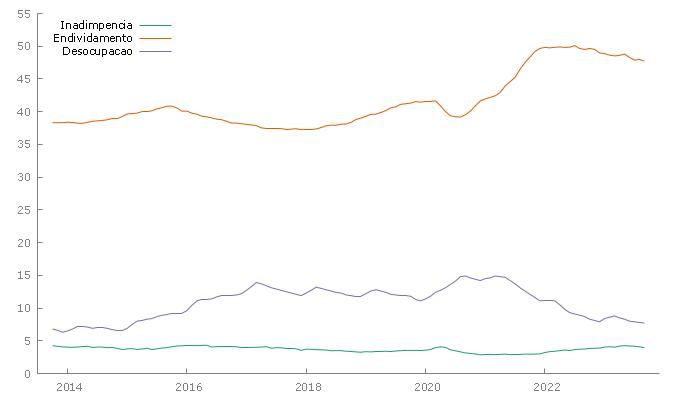
\includegraphics[width=0.8\textwidth]{figs/exemplo.png}\\
{\footnotesize Fonte: Fonte da Imagem}
\end{figure}

\subsection{Metodologia}

Explique como o trabalho foi realizado, apresentando os procedimentos
necessários para compreender como os resultados foram obtidos. Conforme a
natureza da investigação, informe participantes ou amostra, local e período,
materiais e instrumentos, procedimentos, técnicas e métodos de análise.
Apresente somente as informações pertinentes à compreensão e à avaliação da
investigação.

Quando houver formulários, instrumentos de coleta, conjuntos de dados, códigos, documentos ou outros recursos relevantes para a compreensão ou reprodução da pesquisa, esses materiais poderão ser disponibilizados em repositórios públicos, como GitHub, repositórios institucionais ou repositórios de dados científicos.

Sempre que possível, deverão ser utilizados repositórios que ofereçam versionamento, preservação e identificação persistente do material, como DOI. Na versão identificada, o texto deverá indicar claramente a existência desses recursos, apresentar o respectivo link e incluí-los nas referências quando possuírem referência bibliográfica própria.
Durante a avaliação, será considerado exclusivamente o conteúdo apresentado no manuscrito. Portanto, nenhuma informação indispensável à compreensão, fundamentação ou avaliação do trabalho deverá constar apenas nos materiais complementares.

Na versão anônima, os autores poderão mencionar a existência desses materiais, mas deverão omitir links, referências bibliográficas ou outros identificadores que possam revelar a autoria. Essas informações deverão ser acrescentadas somente após a aprovação, na versão identificada.

\begin{itemize}
\item \textbf{Exemplo na versão anônima:} O instrumento de coleta utilizado na pesquisa e os dados brutos anonimizados serão disponibilizados em repositório público na versão identificada do trabalho.
\item \textbf{Na versão identificada:} O instrumento de coleta utilizado na pesquisa e os dados brutos anonimizados estão disponíveis em \url{https://github.com/organizacao/projeto} \cite{instrumento2026}.
\end{itemize}

Para inserir algoritmos, você pode utilizar o seguinte modelo e referenciação \ref{alg:busca_binaria}.

\begin{algorithm}[ht]
\caption{Busca Binária($A$, $x$)}
\label{alg:busca_binaria}
\KwIn{Vetor ordenado $A$, valor $x$}
\KwOut{Índice de $x$ em $A$ ou \texttt{-1}}
$e \leftarrow 1$,\; $d \leftarrow \mathrm{tamanho}(A)$\;
\While{$e \le d$}{
  $m \leftarrow \lfloor (e+d)/2 \rfloor$\;
  \eIf{$A[m] = x$}{
    \Return $m$\;
  }{
    \lIf{$A[m] < x$}{$e \leftarrow m+1$}
    \lElse{$d \leftarrow m-1$}
  }
}
\Return \texttt{-1}\;
\end{algorithm}

Fórmula são apresentadas de forma centralizada e devem ser citadas pela numeração tal como \ref{math:foo}.

\begin{equation}
\label{math:foo}
y_{i,t} = c_i + \phi_{i,1}y_{1,t-1} + \phi_{i,2}y_{2,t-1} + \ldots + \phi_{i,k}y_{k,t-1} + \epsilon_{i,t}
\end{equation}

\subsection{Resultados e Discussão}

Apresente os principais resultados obtidos a partir dos procedimentos
descritos na metodologia. Sempre que possível, utilize indicadores
quantitativos e evidências qualitativas. Não apresente como resultado apenas a
realização de atividades: a atividade descreve o que foi feito, enquanto o
resultado evidencia o que foi obtido ou observado. Em trabalhos ainda em
andamento, apresente os resultados parciais já obtidos.

Discuta os resultados em relação ao problema e aos objetivos do trabalho e,
quando pertinente, à fundamentação teórica e a outros estudos. Interprete os
achados, suas implicações e limitações, evitando apenas repetir os resultados
apresentados.

A Tabela \ref{tab:salario} é um exemplo de como inserir uma Tabela.

\begin{table}[ht]
\caption{Título da Tabela.}
\label{tab:salario}
\centering
\begin{tabular}{lccc}
\toprule
\textbf{Coluna 1} & \textbf{Coluna 2} & \textbf{Coluna 3} & \textbf{Coluna 4} \\
\midrule
Linha 1                    & 03,7027 & 010,832 & 041,526 \\
Linha 2                  & 03,7600 & 011,700 & 039,830 \\
Linha 3                   & 02,8500 & 06,3000 & 037,250 \\
Linha 4                  & 04,3200 & 014,900 & 050,090 \\
\bottomrule
\end{tabular}
\caption*{Fonte: Fonte da Tabela}
\end{table}

\section{Considerações Finais}

Parte final do resumo, na qual se apresentam as considerações correspondentes
aos objetivos e/ou hipóteses.

Retome o objetivo do trabalho e sintetize as principais conclusões a partir dos
resultados apresentados. Destaque as contribuições do trabalho e, quando
pertinente, apresente suas limitações, possibilidades de aplicação dos
resultados e perspectivas para trabalhos futuros. As conclusões devem ser
sustentadas pelos resultados apresentados e não devem introduzir informações,
dados ou argumentos que não tenham sido discutidos anteriormente.

\qcentersection{AGRADECIMENTOS (opcional)}

Agradecimentos a pessoas e/ou instituições, se for o caso, devem ser inseridos após os elementos pós-textuais e de maneira sucinta. Caso o trabalho tenha recebido recursos da Coordenação de Aperfeiçoamento de Pessoal de Nível Superior (Capes), atentar para o que consta na Portaria nº 206, de 4 de setembro de 2018. 

%%%%%%%%%%%%%%%%%%%%%%%%%% REFERÊNCIAS %%%%%%%%%%%%%%%%%%%%%%%%%%%%%%%%

\printbibliography


\end{document}
